\chapter{Algorithms}

\section{Efficient Edge-Preserving Stereo Matching}

This algorithm uses a combination of Sum of Absolute Differences and Census transform as cost for each pixel and a corresponding disparity. Then these costs are aggregated using successive weighted sum and permeability.

Steps:
\begin{enumerate}
\item Calculate cost for each pixel and each disparity
\item Calculate permeability for each pixel
\item Calculate left scan order (right to left direction) for each pixel and disparity
\item Calculate right scan order (left to right direction) and combine it and left scan into horizontal aggregation for each pixel and disparity.
\item Calculate top scan order using horizontal data for each pixel and disparity
\item Calculate bottom scan order using horizontal data and combine it and to scan into total aggregation for each pixel and disparity. 
\item Find minimum among disparity values for each pixel
\end{enumerate}

\subsection*{complexity}
N = number of pixels and d = max disparity value. $0$ = multiplications and division and $\Theta$ = additions and subtractions\\
The cost calculation requires: $(3 \times subtraction + 2 \times additions)$ for each SAD cost.\\
$((Cen_{size}\times Cen_{size} - 1) \times comparisons)$ for each census transform.\\
$(Cen_{size} \times XOR + 1 \times sum)$ for each hamming distance calculation.\\
$2 \times multiplication + 1 \times addition$ for combining costs. \\~\\
\textbf{step 1 total:} $(3\times subtraction + 2 \times addition) \times (d+1) \times N + ((Cen_{size}\times Cen_{size} - 1) \times comparisons) \times (d+2) \times N + (Cen_{size} \times XOR + 1 \times sum) \times (d+1) \times N + (2 \times multiplication + 1 \times addition) \times (d+1) \times N$\\
= $O(2N \times d) + \Theta(6N \times d)$\\~\\

Permeability requires: $4 \times (1 \times minimization + 3 \times (exp + subtraction + div)$ for each pixel\\~\\
\textbf{Step 2 total:} $4 \times (1 \times minimization + 3 \times (exp + subtraction + div) \times N$\\
= $O(12N)+\Theta(12N) + 12 \times exp \times N$\\~\\

Left scan order requires: $1 \times add + 1 \times mult$ for each pixel and disparity\\~\\
\textbf{Step 3 total:} $(1 \times add + 1 \times mult) \times N \times (d+1)$\\
= $O(N\times d) +\Theta(N\times d)$\\~\\

Horizontal + right scan order requires: $2 \times add + 1 \times mult$ for each pixel and disparity\\~\\
\textbf{Step 4 total:} $(2 \times add + 1 \times mult) \times N \times (d+1)$\\
= $O(N\times d) +\Theta(2N\times d)$\\~\\

Top scan order requires: $1 \times add + 1 \times mult$ for each pixel and disparity\\~\\
\textbf{Step 3 total:} $(1 \times add + 1 \times mult) \times N \times (d+1)$\\
= $O(N\times d) +\Theta(N\times d)$\\~\\

Vertical + bottom scan order requires: $2 \times add + 1 \times mult$ for each pixel and disparity\\~\\
\textbf{Step 4 total:} $(2 \times add + 1 \times mult) \times N \times (d+1)$\\
= $O(N\times d) +\Theta(2N\times d)$\\~\\

\textbf{Total cost:} = $O(6N \times d + 12N) + \Theta(12 N \times d + 12 N) + 12 \times exp \times N$

\subsection*{Memory}
input requires: $2 \times N \times d \times 3 \times 8bit + 2 \times N \times d \times 8bit = N \times d \times 64 bit$ \\
step 1 requires: $N \times \times d 32 bit float = N \times d \times 32 bit$\\
step 2 requires: $N \times 4 \times 32 bit float = N \times 128 bit$\\
step 3 requires: $N \times d \times 32 bit float = N \times d \times 32 bit$\\
step 4 requires: $(N \times d + 1) \times 32 bit float = (N \times d + 1)\times 32 bit$\\
step 5 requires: $N \times d \times 32 bit float = N \times d \times 32 bit$\\
step 6 requires: $(N \times d + 1) \times 32 bit float = (N \times d + 1)\times 32 bit$\\
output requires: $N \times \lceil log_2 (d) \rceil bits$

\subsection*{simulation:}
I have coded a simulation of this algorithm in python. Runtime: 184 secs for tsukuba test set (384 x 288 pixels, max disparity value of 30)

\begin{figure}
  \centering
  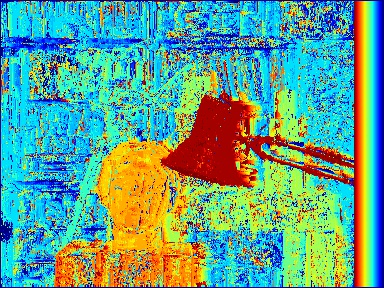
\includegraphics[width=0.5\textwidth]{images/test.jpg}
  \caption{Tsukuba result from EEPSM algorithm}
  \label{fig:eepsmtsu}
\end{figure}

\section{Fast Cost Volume}

This algorithm uses a combination of Sum of Absolute Differences and Gradient as cost for each pixel and a corresponding disparity. Then these costs are weighted by a guided image filter.

\subsection*{complexity}

guided filter is $O(N)$ according to articles.

\subsection*{memory}
mem for 

input requires: $2 \times N \times d \times 3 \times 8bit + 2 \times N \times d \times 8bit = N \times d \times 64 bit$ \\
\subsection*{simulation}
My own python implementation: runtime: 62 for tsukuba test set (384x288 pixels, max disparity value of 30).

\begin{figure}
  \centering
  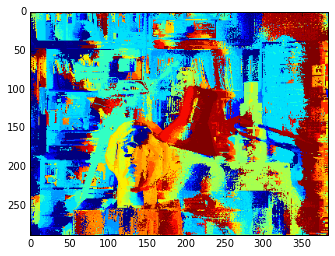
\includegraphics[width=0.5\textwidth]{images/test2.png}
  \caption{pyt test 30}
  \label{fig:my}
\end{figure}

Matlab implementation by authors: runtime: 51 seconds for tsukuba test set (384x288 pixels, max disparity value of 15) and 93 seconds for tsukuba test set (384x288 pixels, max disparity value of 30)

\begin{figure}
  \centering
  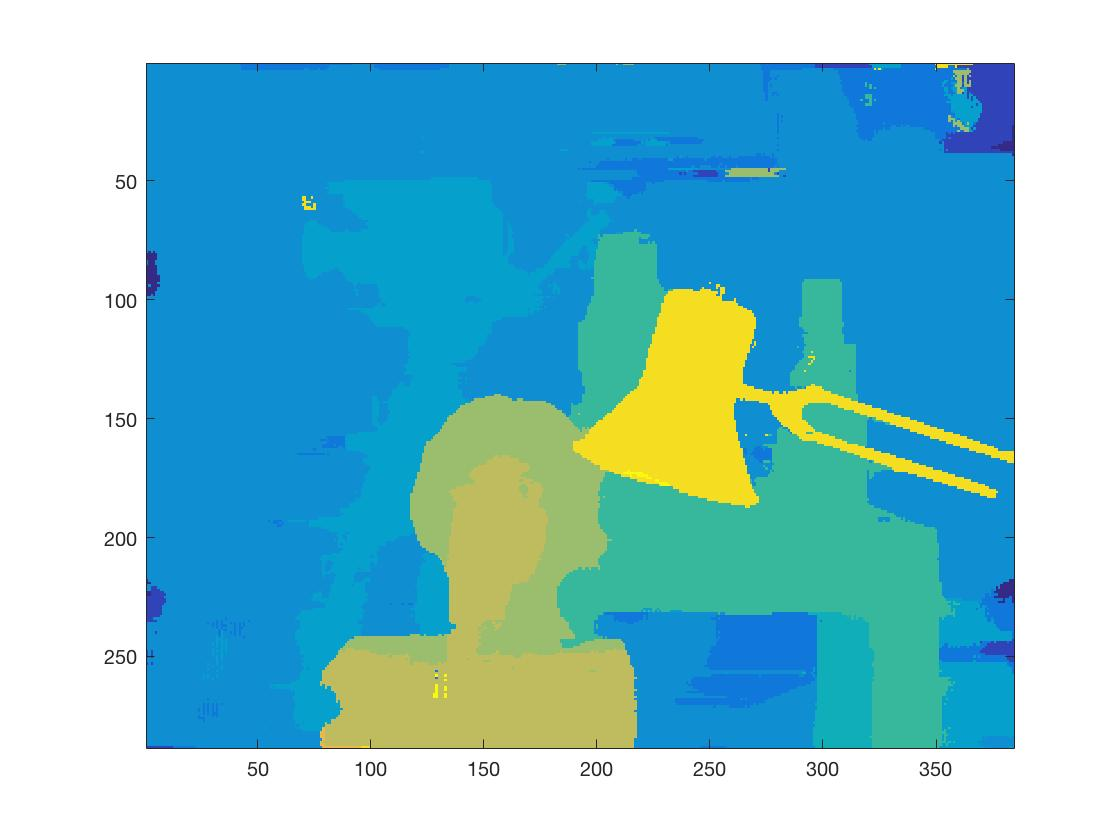
\includegraphics[width=0.5\textwidth]{images/matlabtest.jpg}
  \caption{mat test 15 disp}
  \label{fig:da}
\end{figure}

\begin{figure}
  \centering
  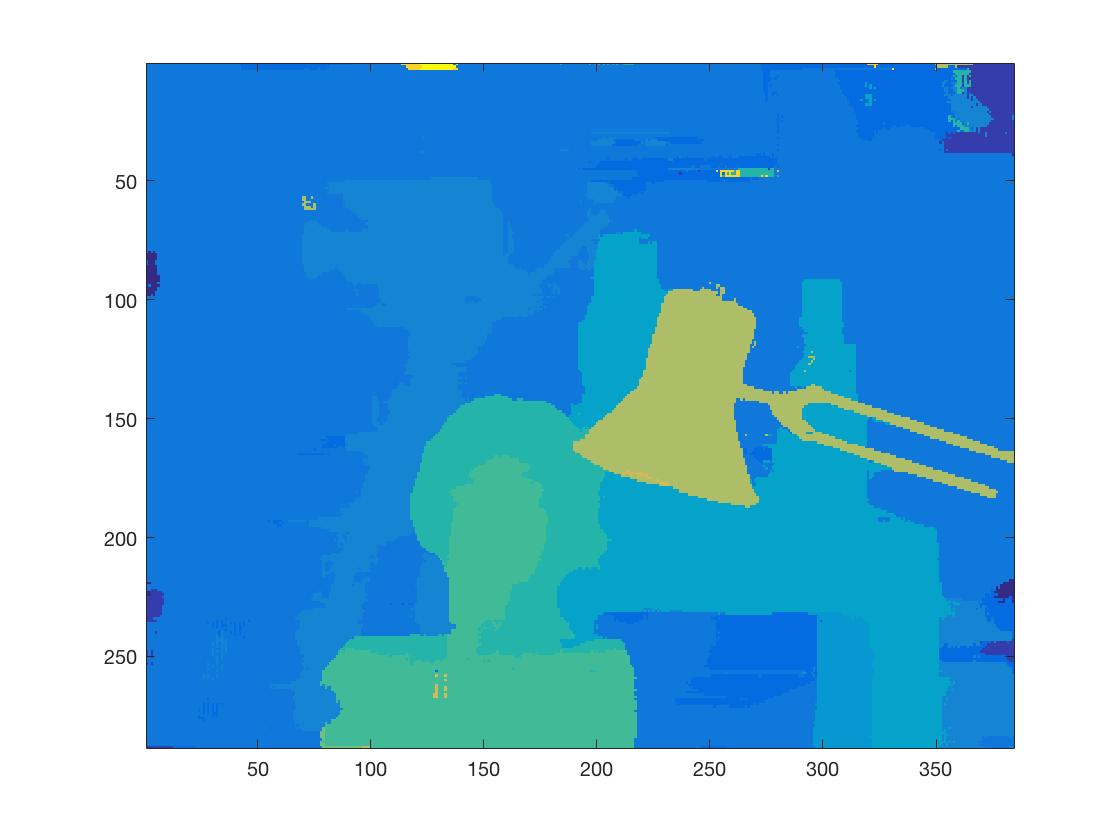
\includegraphics[width=0.5\textwidth]{images/mat2.jpg}
  \caption{mat test 30 disp}
  \label{fig:da2}
\end{figure}

